% For tracking purposes - this is V2.0 - May 2012

\documentclass{sig-alternate}

\usepackage{multirow}
\usepackage{epstopdf}
\usepackage{subfigure}
\usepackage{booktabs}
\usepackage{diagbox}



\begin{document}
\title{Context-aware Sequential Recommendation}

\numberofauthors{4}
\author{
        Anonymous CIKM submission\\
        \\
        Paper ID 22
       }
\maketitle


\begin{abstract}
Sequential information ia becoming a significant factor in modeling user behavior, and various sequential recommendation methods are proposed. As a widely used approach, markov chain based models are constructed on a strong independence assumption. And recurrent neural networks based methods have achieved state-of-the-art performances in sequential modeling. However, recurrent neural networks and other conventional sequential methods are unable to modeling variety of contextual information in complex real-world application, which has been proved to be very important for modeling user behaviors. Meanwhile, existing context-aware recommendation methods also can not take sequential information and temporal dependency into consideration. Thus, it is vital to address and investigate the problem of context-aware sequential recommendation. In this paper, considering the properties of sequential user behaviors, we conclude two types of contexts: input contexts and transition contexts. Input contexts are the situations that user behaviors happen, e.g., time, location and weather. And transition contexts denote time intervals between adjacent behaviors in historical sequences. Based on these information, we propose a novel Context-Aware Recurrent Neural Networks (CA-RNN) model. Instead of the constant input matrix and transition matrix in conventional recurrent neural networks, the corresponding matrices in CA-RNN change according to input contexts and transition contexts respectively. Then, context-specific input matrices and context-specific transition matrices are incorporated and applied. Experimental results show that the proposed CA-RNN model yields significant improvements over the state-of-the-art sequential recommendation methods and context-aware recommendation methods on three typical datasets, i.e., Tmall dataset and Fashion dataset.
\end{abstract}

\keywords{Sequential recommendation, context-awareness, recurrent neural networks} % NOT required for Proceedings

\section{Introduction}
Nowadays, people are overwhelmed by huge amount of information, the exposure to information made people tired of extracting useful and valuable information that they are interested in. This phenomenon turns out to facilitate the development of recommender systems in social networking, e-commerce, online movie and reading websites. Recommender system has now been an important tool for helping people to filter information and locate their preference. Conventional recommendation methods focus on modeling users' preference based on their historical choices of items and always ignore the sequential information. However, user preferences always change with time. Historical behaviors in different time periods have different effects on users' next choice. Accordingly, sequential recommendation is a crucial task for predicting users' next behaviors in recommender sysytems.

Nowadays, the importance of sequential information in recommender system has been gradually recognized by researchers in many disciplines, and some efforts have been put into developing CF methods with sequential information \cite{campos2014time}. Markov Chain (MC) based models \cite{yang2010personalizing,rendle2010factorizing,natarajan2013app,chen2015personalized} have been widely used for sequential prediction. MC based models aim to predict the users' next behavior based on the past behaviors in sequential data. A transition matrix is estimated, which can give the probability of an action based on the previous ones. For personalized recommendation, Factorization Personalized Markov Chain (FPMC) \cite{rendle2010factorizing} provide more accurate prediction by factorizing a personalized transition tensor. However, a major problem of MC based models is that all the components are independently combined, indicating that it makes strong independence assumption among multiple factors. Furthermore, MC based methods have been extended via representation learning, which have been applied to next basket recommendation \cite{wang2015learning}. Recently, as another typical representation learning method, Recurrent Neural Networks (RNN) have been employed to model temporal dependency for different applications successfully. RNN consists of an input layer, an output unit and multiple hidden layers. Hidden representation of RNN can change dynamically along with a sequential history. Each layer of RNN contains an input element and recurrent transition from the previous status, which are captured by an input matrix and a transition matrix respectively. RNN is famous for its being successfully applied in sentence modeling tasks \cite{mikolov2010recurrent,mikolov2011extensions,mikolov2011rnnlm}. It also achieves state-of-the-art performances in sequential click prediction \cite{zhang2014sequential}, location prediction \cite{liu2016strnn} and next basket recommendation \cite{yu2016dream}. Considering its great performances in sequential modeling tasks, RNN is a suitable tool for sequential recommendation.

Though RNN has achieved satisfactory performances, it still has its drawbacks in sequential recommendation situations. Nowadays, with enhanced ability of systems in collecting information, a great amount of contextual information in recommender systems has been collected such as location, time, weather and so on. These kinds of contextual information have significant effect on user behaviors. For instance, a man may like to watch cartoon with his children while may like to watch romantic movies with his wife. He may prefer to read novels during weekend while may tend to read professional books during weekdays. Contextual information has been proved to be useful in determining users' preferences in recommender systems \cite{palmisano2008using,adomavicius2011context}. Context-aware recommendation has been extensively studied and several methods have been proposed to achieve state-of-the-art performances \cite{rendle2011fast,shi2012tfmap,jamali2013heteromf,shi2014cars,liu2015cot}. Without considering the rich contextual information in real world, RNN and other sequential recommendation methods can only model historical sequences and are hard to further improve the performances of recommendation in complex real applications. In contrast, there are also no context-aware recommendation methods that take sequential information into consideration. Unfortunately, as shown in the example in Figure, complex real-world applications usually have both sequential and contextual information. Thus, context-aware recommendation becomes an emerging task, and adapting RNN for variety of contextual information is a good methodology.

To incorporate contextual information in RNN and other sequential models, we investigate the properties of sequential behavioral histories and conclude two types of contexts: \textbf{input contexts} and \textbf{transition contexts}. These two types of contexts are shown in the demonstration in Figure. And we will explain them one by one.

Input contexts denote the contexts of input elements in behavioral sequences, that is to say, input contexts are situations that users conduct behaviors, e.g., shopping, visiting or reading. Such contexts usually include location (home or working place), time (weekdays or weekends, mourning or evening), weather (sunny or rainy) and so on. As we mentioned above, input contexts have significant effects on predicting present behaviors of users. Similarly, input contexts in the history are also useful for predicting the future. For instance, if a man usually takes excise in the morning, then we can predict he will go to the fitting room in the morning rather than evening, even if there are also lots of people going to fitting rooms in the evening.

Transition contexts are the contexts for the transition from previous behaviors in historical sequences. They capture how the previous behaviors affect the future. Specifically, transition contexts denote time intervals between adjacent behaviors in sequences in this paper. Generally speaking, longer time intervals and shorter time intervals means different for the transition from the past. If a user's last behavior on an online shopping website happens half a year ago, then his or her past behaviors have limited effects on the user's future purchasing and a recommendation with popular items may be a better choice. If the user's last behavior happens yesterday, then his or her next purchasing will be significantly affected by the previous ones and a personalized recommendation should be made.

Thus, to model sequential information and contextual information in one framework, we propose a novel model called Context-Aware Recurrent Neural Networks (\textbf{CA-RNN}). Instead of a constant input matrix for capturing input elements in each layer of RNN, we use context-specific input matrices for each specific input contexts. Similarly, we use context-specific transition matrices for modeling transition effects from previous behaviors in historical sequences under specific transition contexts, i.e., time intervals between adjacent behaviors. Then, we implement our CA-RNN model in a Bayesian Personalized Ranking (BPR) \cite{rendle2009bpr} framework to make personalized ranking of recommended items, and Back Propagation Through Time (BPTT) \cite{rumelhart1988learning} is applied for learning parameters of CA-RNN. In summary, the main contributions of this work are listed as follows:

\begin{itemize}
\item
We address the problem of context-aware sequential recommendation, which presents a novel perspective for enhanced recommendation. And we conclude two types of contexts in this problem: input contexts and transition contexts.

\item
We apply context-specific input matrices to model input contexts, which can capture the properties of contextual information in behavior histories and can make context-aware recommendations for users.

\item
We incorporate context-specific transition matrices for modeling transition contexts, i.e., time intervals between adjacent behaviors in historical sequences. This process captures transition effects from the past behaviors to the future behaviors within different time intervals.

\item
Experiments conducted on two real-world datasets show that CA-RNN is effective and clearly outperforms the state-of-the-art methods.

\end{itemize}

The rest of the paper is organized as follows. In section 2, we review some related work on sequential recommendation and context-aware recommendation. Then we give the formulation of context-aware sequential recommendation in section 3. Section 4 details our CA-RNN model. In section 5, we introduce the learning methods of our proposed model. In section 6, we conduct experiments in two real-world datasets and compare with several state-of-the-art methods. Section 7 concludes our work and discusses future research.


\section{Related Works}
In this section, we review some related works on sequential recommendation and context-aware recommendation.

\subsection{Sequential Recommendation}

Time-aware neighbourhood models \cite{ding2005time,lathia2009temporal,liu2010online} may be the most natural methods for modeling sequences, which employ neighbourhood based algorithms to capture temporal effects via giving more relevance to recent observations and less to past observations. Using frequent pattern mining, sequential pattern based methods \cite{mobasher2002using,hariri2012context} seek sequential patterns that occur most frequently to predict the future. However, both neighbourhood based and sequential pattern based methods are unable to reveal the underlying properties in users' historical sequences. And sequential pattern based methods are time consuming in large scale datasets.

Matrix factorization based methods \cite{koren2009matrix} have become the state-of-the-art approach to conventional recommendation, which have been extended to time-aware factorization based models recently. Tensor Factorization (TF) \cite{xiong2010temporal,bahadori2014fast} treats time intervals as another dimension and generate latent vectors of time intervals via factorization to capture the underlying properties in historical sequences. TimeSVD++ \cite{koren2010collaborative} learns time-aware representations for users and items. However, factorization based models have difficulties in generating latent representations for time intervals which has never or seldom appeared in the training data.

The MC based methods are widely used models for sequential applications \cite{yang2010personalizing}. Via factorization of the probability transition matrix, Factorizing Personalized Markov Chain (FPMC) \cite{rendle2010factorizing} can provide more accurate prediction for each sequence. FPMC is also extended by using user group \cite{natarajan2013app} or incorporating location constraint \cite{cheng2013you}. Recently, some factors of human brain have been added into MC based methods, including interest-forgetting curve \cite{chen2015personalized} and dynamics of boredom \cite{kapoor2015just}. However, the main drawback of MC based models is the independent combination of the past components, which lies in a strong independence assumption and confines the prediction accuracy. MC based methods are then extended by representation learning. Hierarchical Representation Model (HRM) \cite{wang2015learning} learns the representation of behaviors in the last transaction and predicts behaviors for the next transaction. And Personalized Ranking Metric Embedding (PRME) \cite{feng2015personalized} learns embeddings of users according to the location distance.

Recently, a few prediction models, especially language models, are proposed based on neural networks. The most classical language model is proposed via a single layer neural network \cite{bengio2003neural}. And models based on RNN have been successfully used in modeling sentences \cite{mikolov2010recurrent,mikolov2011extensions,mikolov2011rnnlm}. RNN also brings satisfying results for sequential click prediction for sponsored search \cite{zhang2014sequential}, location prediction \cite{liu2016strnn} and next basket recommendation \cite{yu2016dream}. RNN is showing its great performances in sequential modeling.

\subsection{Context-aware Recommendation}

Context-aware recommender system (CARS) \cite{adomavicius2011context} generates more relevant recommendations by adapting them to the specific contextual situation of the user, and it built based on the knowledge of contextual user preferences and typically deal with data records of user, item and context. Recent works on contextual modeling approaches extend the user-item preference relations with contextual information and incorporate factorization models to compute recommendations. Multi-verse recommendation \cite{karatzoglou2010multiverse} uses tensor factorization to model n-dimensional contextual information. The social network aided context-aware recommender system \cite{liu2013soco} splits contexts and performs general matrix factorization on each leaf of decision trees. As a extended model of tensor factorization, Factorization Machine (FM) \cite{rendle2011fast} can model a wide variety of contextual information by specifying contextual information as the input dimensions and provide context-aware predictions. The work on Heterogeneous Matrix Factorization (HeteroMF) \cite{jamali2013heteromf} generates context-specific latent vectors of entities using a context-dependent transfer matrix and the original latent vectors of entities. The Tensor Factorization for MAP maximization (TFMAP) model \cite{shi2012tfmap} uses tensor factorization and Mean Average Precision (MAP) objective to model implicit feedback data with contextual information. The newly CARS2 \cite{shi2014cars} and Contextual Operating Tensor (COT) \cite{liu2015cot} models represent the common semantic effects of contexts as contextual operating tensor and represents contexts as latent vectors. And the Hierarchical Interaction Representation (HIR) model \cite{liu2015collaborative} generates the interaction representation via tensor multiplication which can be applied in context-aware recommender system.

\section{Proposed Model}

% \begin{figure*}[htb]
% \centering
% 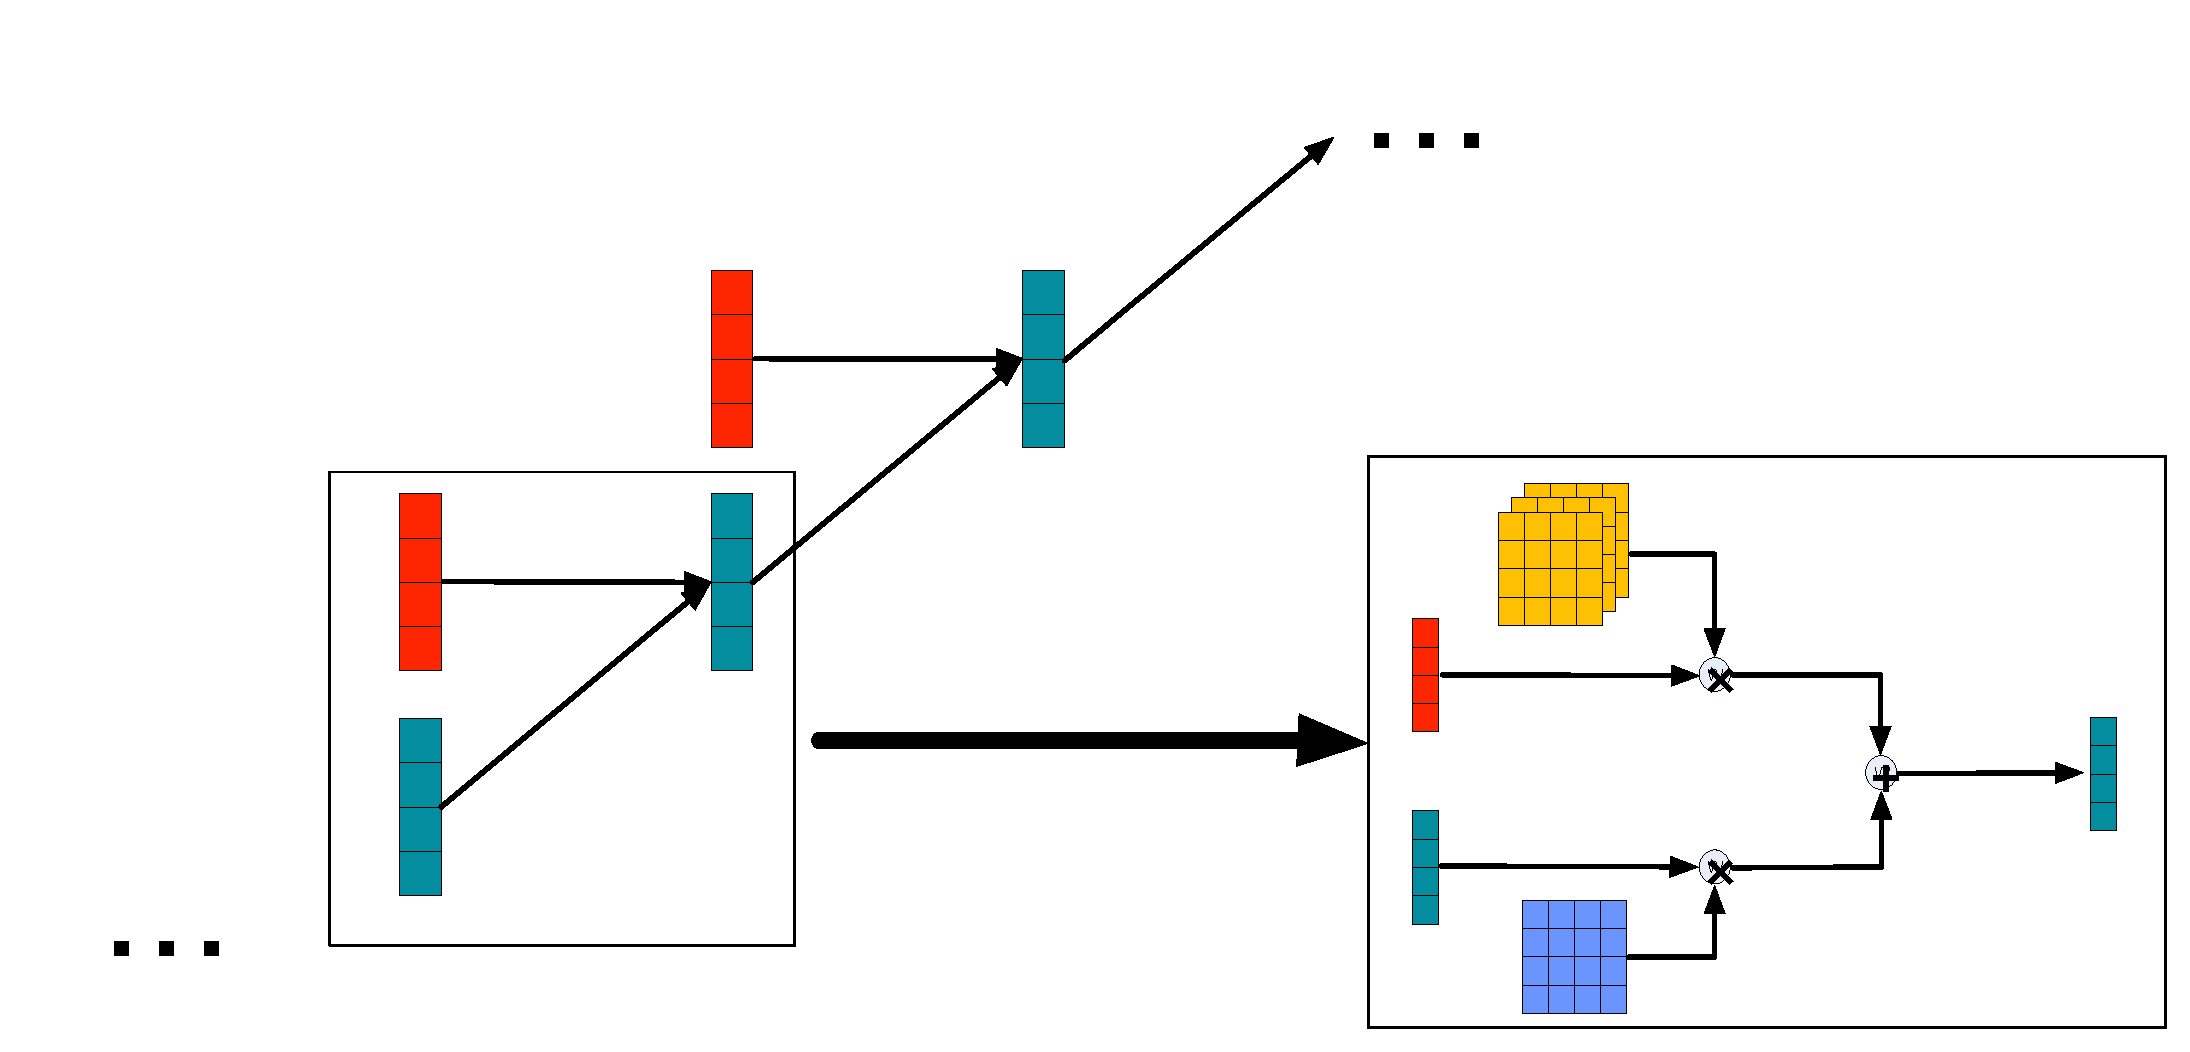
\includegraphics[width=1\linewidth]{./model.pdf}
% \caption{The model}
% \label{fig:Model-overview}
% \end{figure*}

\subsection{Problem Formulation}
We have a set of users denoted as $U  = \{ u_1 ,u_2 ,...\}$, a set of items denoted as $V  = \{ v_1 ,v_2 ,...\}$. There are multiple input contexts denoted as $C^I = \{c_{i1} ,c_{i2} ,...\}$, such as weather, location, mood and so on. Meanwhile, each context contains several conditions. For example, mood context may consist of happy, sad and flat. The transition context $C_t$ accounts for the different time interval between two records of user. For each user $u$, the behavioral history is given as $V^u = \{v^u_{1}, v^u_{2}, ...\}$, where $v^u_{i}$ denotes the $i$ th selected item of user. And the history of all users is denoted as $V^U = \{V^u_{1}, V^u_{2}, ...\}$. The behavioral history is associated with corresponding timestamps $T^u = \{t^u_{1}, t^u_{2}, ...\}$ where $t_k$ denotes the $k$ th timestamp in one sequence. For each user $u$, at specific timestamp $t_k$, a combination of input contexts is denoted as $\{
c_{i1,k}^{u},c_{i2,k}^{u},...\}$.


\subsection{ Recurrent Neural Networks}
The architecture of a recurrent neural network consists of an input layer $i$, a hidden layer $h$, an output unit, as well as inner weight matrices \cite{zhang2014sequential}. RNN model the current output as the function of the previous output and a hidden layer. At each time steps, we can predict the output unit given the hidden layer, and then feed the new output back into the next hidden state. The vector representation of the hidden layer is:
\begin{equation}
\mathbf{h}_{k}^{u}=f\left ( {\mathbf{r}_{v_{k}^{u}}}\mathbf{M}+\mathbf{h}_{k-1}^{u}\mathbf{W} \right),~
\end{equation}
where $\mathbf{h}^u_{k}$ is the $d$ dimensional representation of  user $u$ at time $k$ in a behavior sequence, $\mathbf{r}_{v_{k}^{u}}$ denotes the $d$ dimensional latent vector of the corresponding item the user selects, $\mathbf{W}$ is the $d \times d$ dimensional recurrent connection of the previous status propagating sequential signals and $\mathbf{M}$ denotes the $d \times d$ dimensional transition matrix for input elements to capture the current behavior of the user. The activation function $f(x)$ is chosen as a $sigmoid$ function $f(x) = \exp \left( {1 \mathord{\left/ \right. \kern-\nulldelimiterspace} 1 + e^{ - x} } \right)$.

\subsection{ Incorporating Transition Context}
Since the shorter the time interval is, the more accurate the prediction will be. The length of time interval between two statues have different impact on the prediction, we incorporate Transition Context in the formula. We replace the transition matrix $\textbf{W}$ with type-specific transition matrices. Thus, Equation should be rewritten as: 
\begin{equation}  \label{eqh}
\textbf{h}_{k}^{u}=f\left ( \textbf{r}_{v_{k}^{u}}\textbf{M}+\textbf{h}_{k-1}^{u}\textbf{W}_{ t_k^u-t_{k-1}^u  }\right )
~\end{equation}
 where $t_k^u$ and $t_{k-1}^u$ denotes the present and the previous statues respectively, $t_k^u-t_{k-1}^u$ is the time interval.  All kinds of time intervals are continuously classified into several types according to their length. We suppose that each type should contain near the same quantity of different time intervals. Then, Equation should be rewritten as: 
\begin{equation}
\textbf{h}_{k}^{u}=f\left ( \textbf{r}_{v_{k}^{u}}\textbf{M}+\textbf{h}_{k-1}^{u}\textbf{W}_{\left\lfloor t_k^u-t_{k-1}^u \right\rfloor }\right )
~\end{equation}
where $\left\lfloor t_k^u-t_{k-1}^u \right\rfloor$ denotes for the type of the time interval between $t_k^u$ and $t_{k-1}^u$ .




\subsection{ Context-aware Recurrent Neural Networks}
Since context information is important in future predictions and conventional RNN cannot model it, it is essential to involved context information in our model. Thus, we add the input context $c_{I,k}^{u}$ to the transition matrix $\textbf{M}$ in traditional RNN model. In CA-RNN model, given a user $u$, his or her vector representation at time $k$ can be calculated by using an integrated contextual operating matrix for a specific context combination. This matrix describe how a context combination affects the properties of entities and how context-specific latent vectors of users and items can be generated from their original ones. Here, we can calculate context-specific latent vectors as: 
\begin{equation}
\textbf{h}_{k}^{u}=f\left ( \textbf{r}_{v_{k}^{u}}\textbf{M}_{c_{I,k}^{u}}+\textbf{h}_{k-1}^{u}\textbf{W}_{\left\lfloor t_k^u-t_{k-1}^u \right\rfloor }\right )
~
\end{equation}
where  $\textbf{W}$ is a $d*d$ dimensional transition matrix from the last status, $\textbf{r}_{v_{k}^{u}}$ is a  $d$ dimensional vector representation of the input item at time $k$ of user $u$, and $\textbf{M}_{c_{I,k}^{u}}$ is a  $d*d$ transition matrix of correspondence context, denoting the aggregation of all contextual operating matrices for users and items under the context combination . 


Linear computation is another common method to calculate the aggregation of all contextual operating matrices, It treats the effect of each context seperately, the $\textbf{M}_{c_{I,k}^{u}}$ can be calculated as:
\begin{equation} \label{eqMadd}
\textbf{M}_{c_{I,k}^{u}} = \sum_{c_{i,k}^{u}\in C^I} \textbf{M}_{c_{i,k}^{u}} 
~
\end{equation}

Nonlinear method incorporates sigmoid function to the computation, such as tanh or logistic funtion. Accordingly, the equation could be rewritten as :
\begin{equation}
\textbf{M}_{c_{I,k}^{u}} ={ \left(1+\exp \left(-\sum_{c_{i,k}^{u}\in C^I} \textbf{M}_{c_{i,k}^{u}}  \right) \right)}^{-1}
~
\end{equation}


In STRNN  \cite{liu2016strnn} ,the author incorporates temporal and spatial contexts into conventional RNN by mutipling time-specific operating matrix and distance-specific operating matrix. Analogously, we can treat input contextual operating matrices in the same way :
\begin{equation}
\textbf{M}_{c_{I,k}^{u}} = \prod_{c_{i,k}^{u}\in C^I} \textbf{M}_{c_{i,k}^{u}} 
~
\end{equation}

Moreover, the $\textbf{M}_{c_{I,k}^{u}}$ can be a combination-specific matrix. For example, if there are two contexts: weather and mood, then each context combination has its own matrix as shown in table 1. From a set of matrices for all combinations, the $\textbf{M}_{c_{I,k}^{u}}$ will be chosen as the representation for specific context combination at time $k$. If the weather is sunny and mood is happy, then the  $\textbf{M}_{c_{I,k}^{u}}$ will equal to $\textbf{M}_{11}$.

\begin{table}[!htbp]
\caption{}
\centering
\begin{tabular}{|l|r|l|r|}
\hline
\diagbox{Weather}{Mood}&happy&sad&plain\\
\hline
sunny&$\textbf{M}_{11}$&$\textbf{M}_{12}$&$\textbf{M}_{13}$\\
\hline
rainy&$\textbf{M}_{21}$&$\textbf{M}_{22}$&$\textbf{M}_{23}$\\
\hline
cloudy&$\textbf{M}_{31}$&$\textbf{M}_{32}$&$\textbf{M}_{33}$\\
\hline
\end{tabular}
\end{table}


\subsection{Context-aware Prediction}

Finally, the prediction of CA-RNN can be yielded via calculating inner product of user and item representations. The prediction of whether user $u$ purchase item $v$  under context $c$ at status $k+1$ can be computed as:
\begin{equation}
y_{u, k+1, c, v} = \mathbf{h}_{k}^{u}\mathbf{P}_{c, k+1}(\mathbf{r}_{v})^ \mathrm{ T }~
\end{equation}
where $\mathbf{P}_{c, k+1}$ is the representation of input context and transition context at status $k+1$. And it can be calculated by the addition or multiplication of $\mathbf{M}^{'}$ and $\mathbf{W}^{'}$ , the corresponding matrix of the two kinds context . Unlike $\mathbf{M}$ and $\mathbf{W}$ in equation 4, which are transition matrices, $\mathbf{M}^{'}$ and $\mathbf{W}^{'}$ are designed for incorporating context information to improve the predicting process. According to our experiments, addition performances better, so $\mathbf{P}_{c, k+1}$ can be calculated as:
\begin{equation}   \label{eqPadd}
\mathbf{P}_{c, k+1}=\mathbf{M}_{c_{I,k+1}^{u}}^{'} + \mathbf{W}_{\left \lfloor t_{k+1}^{u} - t_{k}^{u}\right \rfloor}^{'}~
\end{equation}
where $\mathbf{M}_{c_{I,k+1}^{u}}^{'}$ is the represntation of specific input contexts combination for user $u$ at time $k$ , and $\mathbf{W}_{\left \lfloor t_{k+1}^{u} - t_{k}^{u}\right \rfloor}^{'}$ is the represntation of transition context for interval between the current and the next status. These matrices indicate the effect of current context to the following behavior.




\subsection{Parameter Learning}

In this subsection, we introduce the learning process of CA-RNN with Bayesian Personalized Ranking (BPR) \cite{rendle2009bpr} and Back Propagation Through Time (BPTT) \cite{rumelhart1988learning}.
BPR is a state-of-the-art pairwise ranking framework for the implicit feedback data. The basic assumption of BPR is that a user prefers a selected item than a negative one. Thus, the training objective of CA-RNN in BPR framework is to maximize the following probability:
\begin{equation}
p(u, k+1, c, v\succ v') = g(y_{u, k+1, c, v} - y_{u, k+1, c, v'}),~
\end{equation}
where $v'$ denotes a negative item sample, and $g(x)$ is a nonlinear function which is selected as $g(x) = {1 \mathord{\left/ \right. \kern-\nulldelimiterspace} 1 + e^{ - x}}$. Incorporating the negative log likelihood, we can solve the following objective function equivalently:
\begin{equation}
J = \sum \ln(1+e^{-(y_{u,k+1,c,v} - y_{u,k+1,c,v'})})+\frac{\lambda }{2}\left \| \Theta  \right \|^{2}  ~,
\end{equation}
where $\lambda = {R, M ,W}$ denotes all the parameters to be estimated, $\lambda$ is a parameter to control the power of regularization. And the derivation of $J$ with respect to the parameters can be calculated as: 
\begin{displaymath}
\frac{\partial J}{\partial \mathbf{r}_{v}} = -\sum \frac{\mathbf{h}_{k}^{u}\mathbf{P}_{c,k+1}e^{-(y_{u, k+1, c, v} - y_{u, k+1, c, v'})}}{1+e^{-(y_{u, k+1, c, v} - y_{u, k+1, c, v'})}}+\lambda \mathbf{r}_{v}  ~,
\end{displaymath}
\begin{displaymath}
\frac{\partial J}{\partial \mathbf{r}_{v'}} = \sum \frac{\mathbf{h}_{k}^{u}\mathbf{P}_{c,k+1}e^{-(y_{u, k+1, c, v} - y_{u, k+1, c, v'})}}{1+e^{-(y_{u, k+1, c, v} - y_{u, k+1, c, v'})}}+\lambda \mathbf{r}_{v'}  ~,
\end{displaymath}
\begin{displaymath}
\frac{\partial J}{\partial \mathbf{h}_{k}^{u}} = -\sum \frac{\mathbf{r}_{v}(P_{c,k+1})^{\mathrm{ T }}e^{-(y_{u, k+1, c, v} - y_{u, k+1, c, v'})}}{1+e^{-(y_{u, k+1, c, v} - y_{u, k+1, c, v'})}}   ~,
\end{displaymath}
\begin{displaymath}
\frac{\partial J}{\partial \mathbf{P}_{c,k+1}} = -\sum \frac{(h_{k}^{u})^{\mathrm T}r_{v}e^{-(y_{u, k+1, c, v} - y_{u, k+1, c, v'})}
}{e^{-(y_{u, k+1, c, v} - y_{u, k+1, c, v'})}}    ~.
\end{displaymath}

Moreover, parameters in CA-RNN can be further learnt with the BPTT algorithm. According to Equation \eqref{eqh}, given the derivation ${\partial J \mathord{\left/ \right. \kern-\nulldelimiterspace} {\partial \mathbf{h}_{k}^{u} } }$, the corresponding gradients of all parameters in the hidden layer can be calculated as: 
\begin{displaymath}
\frac{{\partial J}}{{\partial \mathbf{h}^u_{k-1} }} =  \left( {f'\left(  \cdot  \right) \otimes \frac{{\partial J}}{{\partial \mathbf{h}^u_{k} }}} \right)\left({\mathbf{W}_{\left \lfloor t_{k}^{u} - t_{k-1}^{u} \right \rfloor}}\right)^\mathrm{T} ~,
\end{displaymath}

\begin{displaymath}
\frac{{\partial J}}{{\partial {\mathbf{W}_{\left \lfloor t_{k}^{u} - t_{k-1}^{u} \right \rfloor}} }} =  \left({\mathbf{h}_{k-1}^u}\right)^\mathrm{T}\left( {f'\left(  \cdot  \right) \otimes \frac{{\partial J}}{{\partial \mathbf{h}^u_{k} }}} \right) ~,
\end{displaymath}

\begin{displaymath}
\frac{{\partial J}}{{\partial \mathbf{r}_{v_k^u} }} =  \left( {f'\left(  \cdot  \right) \otimes \frac{{\partial J}}{{\partial \mathbf{h}^u_{k} }}} \right)\left({\mathbf{M}_{c^u_{I,k+1}}}\right)^\mathrm{T} ~,
\end{displaymath}

\begin{displaymath}
\frac{{\partial J}}{{\partial {\mathbf{M}_{c^u_{I,k+1}}} }} =  \left({\mathbf{r}_{v^u_k}}\right)^\mathrm{T}\left( {f'\left(  \cdot  \right) \otimes \frac{{\partial J}}{{\partial \mathbf{h}^u_{k} }}} \right) ~.
\end{displaymath}
This process can be repeated iteratively in the whole behavioral sequence. 
Then, according to Equation \eqref{eqMadd} and \eqref{eqPadd}, given ${\partial J \mathord{\left/ \right. \kern-\nulldelimiterspace} {\partial \mathbf{P}_{c,k+1} } }$, the gradients of $\mathbf{M}_{c^u_{i,k+1}}$ and $\mathbf{W}_{\left \lfloor t_{k+1}^{u} - t_{k}^{u} \right \rfloor}$ can be computed as: 
\begin{displaymath}
\frac{{\partial J}}{{\partial {\mathbf{M}_{c^u_{I,k+1}}} }} =  \frac{\partial J}{\partial \mathbf{P}_{c,k+1}} ~,
\end{displaymath}
\begin{displaymath}
\frac{{\partial J}}{{\partial {\mathbf{W}_{\left \lfloor t_{k+1}^{u} - t_{k}^{u} \right \rfloor}} }} =  \frac{\partial J}{\partial \mathbf{P}_{c,k+1}} ~,
\end{displaymath}
\begin{displaymath}
\frac{{\partial J}}{{\partial {\mathbf{M}_{c^u_{i,k+1}}} }} =  \frac{\partial J}{\partial \mathbf{M}_{c^u_{I,k+1}}} ~.
\end{displaymath}
Now, after calculating all the gradients, we can employ stochastic gradient descent to estimate the model parameters. 

\section{Experiments}

\section{Conclusions and Future Work}

In this paper, we have address the problem of context-aware sequential recommendation and proposed a novel method, i.e., context-aware recurrent neural networks. In CA-RNN, the constant input matrix of conventional RNN is replaced with context-specific input matrices to modeling complex real-world contexts, e.g., time, location and weather. Meanwhile, to model transition contexts, i.e., time intervals between adjacent behaviors in historical sequences, contexts-specific transition matrices are incorporated, instead of the constant one in conventional RNN. Then, to make personalized ranking of recommended items, we implement CA-RNN in the BPR framework and apply BPTT to learn parameters in CA-RNN. The experimental results on two real datasets show that CA-RNN outperforms the state-of-the-art sequential and context-aware recommendation models.

In the future, we can further investigate the following direction. In CA-RNN, parameters are the same for different users, which does not confirm to practical situations. So, to make better personalized recommendation,+ we need to find a method to determine different parameters for different users or different user groups. Moreover, we didn't take items' features, e.g., categories, descriptions and images of items, into consideration. Thus, incorporating our CA-RNN with features of items may also be our next step.

\small
\bibliographystyle{abbrv}
\bibliography{sigproc}
\vspace{2cm}

\balancecolumns
\end{document}
